\chapter{CellTAN: Cellular Time Activation Networks} \label{chap:chap4}

This chapter proposes a new tool called CellTAN (Cellular Time Activation Networks) that can effectively address the challenges of distributed information systems characterized by time series data. CellTAN represents sparse yet interconnected components that function independently, cooperatively, and asynchronously. The primary purpose is to identify incoherent components and possible faults effectively. However, the following proposals will introduce other valuable features that come naturally from fulfilling the main objective. 

While initially designed for photovoltaic (PV) systems, the concepts of cells, connections, neighbors, time series, and uncertainty are universal and applicable to other fields such as biology, physics, and more.
Inspired by other effective mechanisms like GNNs, CXNs, and Weighted Cross-Connection Networks (WCCNs), CellTAN uses a graph-like structure to represent a network of components. This structure allows for decentralized knowledge and requires minimal resources for each component to operate in real time.
The subsequent sections of this chapter will explain the working of the "cell" and its interactions within the network, offering a comprehensive understanding of the tool.

\section{Glossary}

\begin{itemize}
    \item \textbf{Knowledge base}: refers to registered historical knowledge (samples) of time series variables.
    
    \item \textbf{Inputs}: a set of variables that define the state of a cell. Instantaneous values, represented by uniform fuzzy numbers.

    \item \textbf{Outputs}: similar to inputs, but obtained through certain computations.

    \item \textbf{Time decay}: a process associated with increased uncertainty of variables over time.
    
    \item \textbf{Time Activations}: a series of time intervals defined by start and end timestamps.

    \item \textbf{Hub}: the central component of the cell network, which facilitates its visualization, management, and expansion. It acts as the proxy agent between the cell's communication.
    
\end{itemize}

\section{The Cell}

A cell is an independent entity composed of \textbf{data} and \textbf{processes}. As an individual part of the system, it follows a set of rules that define its intrinsic and extrinsic behavior. These rules address data privacy, request boundaries, rights, duties, and real-world operational limitations.

\paragraph*{Independence} During operation, dependence on neighbors or other network entities for continuous processing of outputs results in a less robust system and decreases availability. Thus, the cell shall be independent of its surroundings and continue operating in an isolated state given connection cutoffs. This, of course, is not its preferred state, but enduring isolation until outside contact is re-established avoids shutdown and startup procedures. 

\paragraph*{Selfish Computations} The cell is selfish in that it will not perform any computations based on the request of others. This aspect creates a fundamental layer of protection against overloading the infrastructure in which it is deployed, increasing availability.

\paragraph*{Selfless Data} Although selfish in computations, the cell shall provide access to a select set of data useful to the network.

\subsection{Cell's Core}

\subsubsection{Temporal similarity extraction}

Temporal similarity extraction is essential for identifying recurring patterns in time series data. It involves the identification of past instances where the current state is observed to extract useful information about the system's behavior over time. By identifying historical periods with similar states, temporal similarity extraction can help assess the current state or predict future trends. This technique is prized in finance, medicine, and environmental science, where accurate forecasting is critical for effective planning and management. However, the process of temporal similarity extraction can be challenging due to the complexity and size of time series data, as well as the need to accurately measure and compare similarity across different periods.

One approach to simplifying the process of temporal similarity extraction in multi-variate time series data is to use uniform fuzzy values to filter historical data. This technique involves assigning fuzzy membership values to each data point in the time series based on its similarity to the current state. The use of fuzzy values can capture the inherent uncertainty in time series data, making the approach robust to noisy or incomplete data. Moreover, uniform fuzzy values make filtering history trivial and easily streamlined/automated.


\paragraph{Self Similarity}

Having a knowledge base, the cell is capable of performing temporal similarity extraction with itself, using its input variables. When filtering its historical data with two or more variables, there will be a tendency of narrowing down the activated timestamps, which can be utilized to infer a range of more probable uncertainty.

From now on, equations refering to the time variable $t$ assumes that present time is equal to $t=0$. Uniform fuzzy variables will have the notation $x^$.


To demonstrate this process, consider the a cell that is characterized by two variables, which are a function of time: $x(t)$ and $y(t)$. 
Assume that, at a given instant, these are the new cell inputs:

\begin{equation*}
    x(0) = 1.0 \rightarrow x(0) \subset [0.9, 1.1]
\end{equation*}

\begin{figure}[h!]
    \centering
    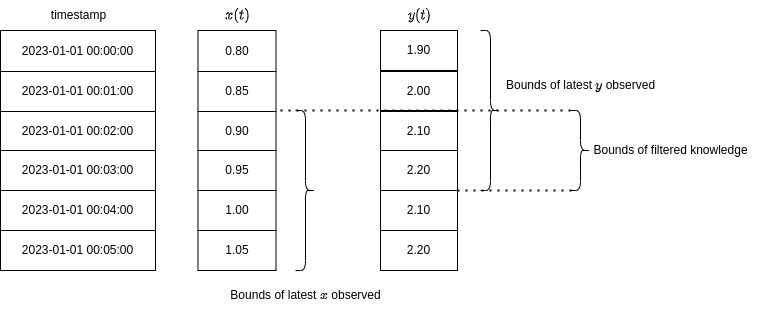
\includegraphics[width=15cm]{figures/chapter4/cell/solo_state_estimation.png}
    \caption{Visualization of self similarity extraction example.}
    \label{fig:solo_state_estimation}
\end{figure}

\paragraph{Mutual Similarity}
Capacidade de estimação de estado intrínsica + extrínsica

\subsection{Connections and Trust}
O que é uma conexão, como se caracteriza, e que valores tem a ela associada
